\documentclass[a4paper]{article}
\usepackage{ulem}
\usepackage{graphicx}
\usepackage[namelimits]{amsmath}
\usepackage{amssymb}
\usepackage{amsmath}
\usepackage{amsfonts}
\usepackage{mathrsfs}
\usepackage{enumerate}
\usepackage{indentfirst}
\usepackage{multirow}
\usepackage{latexsym}
\usepackage{subfig}
\usepackage{listings}
\usepackage{xcolor}
\usepackage{algorithm}
\usepackage{algpseudocode}
\usepackage{forest}

\lstset{numbers=left,
	numberstyle=\tiny,
	frame=shadowbox,
	backgroundcolor=\color[RGB]{245,245,244},
	keywordstyle=\color[RGB]{40,40,255},
	numberstyle=\footnotesize\color{darkgray},
	commentstyle=\color[RGB]{50,50,50},
	breaklines=true,
	tabsize=4,
	showspaces=false}

\renewcommand{\algorithmicrequire}{\textbf{Input:}}
\renewcommand{\algorithmicensure}{\textbf{Output:}}

\title{UM-SJTU JOINT INSTITUTE\\VE477 Introduction to Algorithms\\\vspace{0.5cm} Homework 3}
\author{Li Yong 517370910222}
\begin{document}
\maketitle
\newpage

\section*{Ex.1 Hamiltonian path}
\begin{enumerate}
	\item Depth-first search is an algorithm for traversing or searching tree or graph data structure. The algorithm starts at the root node (or selecting some arbitrary node as the root node in the case of a graph) and explores as far as possible along each branch before backtracking.\par
	Time complexity: $\mathcal{O}(|V| + |E|)$
	\begin{algorithm}
		\caption{Depth-first search}
		\begin{algorithmic}[1]
			\Require $G(E,V)$
			\Ensure DFS path
			\State Let $S$ be a stack
			\State $S$.push($v$)
			\While{$S$ is not empty}
				\State $v\leftarrow S$.pop()
				\If{$v$ is not explored}
					\State Set $v$ is explored
					\For{all adjacent nodes $u$ of $v$}
						\State $S$.push($u$)
					\EndFor
				\EndIf
			\EndWhile
		\end{algorithmic}
	\end{algorithm}
	\item Topological sorting for Directed Acyclic Graph (DAG) is a linear ordering of vertices such that for every directed edge $(u, v)$, vertex $u$ comes before $v$ in the ordering. Topological sorting can be only applied on DAG.\par
	Time complexity: $\mathcal{O}(|V|+|E|)$
	\begin{algorithm}
		\caption{Topological sorting}
		\begin{algorithmic}[1]
			\Require $DAG(E,V)$
			\Ensure A linked list of ordered vertexes.
			\State Call DFS to compute finishing times $v.f$ for each vertex $v$ in $DAG$
			\State As each vertex is finished, insert it into the front of a linked list
			\State\Return The link list
		\end{algorithmic}
	\end{algorithm}
	\item
	\begin{algorithm}
		\caption{Hamiltonian path}
		\begin{algorithmic}[1]
			\Require $DAG(E,V)$
			\Ensure If $DAG(E,V)$ contains a Hamiltonian path
			\State Call Topological sorting to get all results
			\State As each result is got, check if the first and the last node in the linked list are adjacent
			\If{there exists one result satisfies}
				\State \Return True
			\EndIf
			\State \Return False
		\end{algorithmic}
	\end{algorithm}
	\item The number of results of topological sorting must be less than $|V|+|E|$, hence time complexity is $\mathcal{O}((|V|+|E|)^2)$.
	\item $\mathcal{NP}$-complete

\section*{Ex.2 Critical thinking}
	\begin{enumerate}
		\item No. Plot the function, the figure skews exponentially.
		\item $$\frac{\log^*\log{n}}{\log{\log^*{n}}} = \frac{\log^*{n}-1}{\log{\log^*{n}}}$$
		Let $t=\log^*{n}$, then
		$$\frac{\log^*\log{n}}{\log{\log^*{n}}} = \frac{t-1}{\log{t}}$$
		Hence, $\log^*\log{n}$ is asymptotically larger than $\log{\log^*{n}}$.
		\item
		\begin{algorithm}
			\caption{The lighter ball}
			\begin{algorithmic}[1]
				\Require 8 balls, one of which is lighter than others
				\Ensure The lighter ball
				\State Compare 6 balls by balance, each side of 3
				\If{the balance is balanced}
					\State Compare the left 2 balls
					\State \Return the lighter ball
				\Else
					\State Compare 2 of the 3 balls which are lighter
					\If{the balance is balanced}
						\State \Return the left 1 ball
					\Else
						\State \Return the lighter ball
					\EndIf
				\EndIf
			\end{algorithmic}
		\end{algorithm}
	\end{enumerate}
\end{enumerate}

\section*{Ex.3 Rubik’s Cube}
A Rubik's cube is a mechanical puzzle in the shape of a 3$\times$3 cube which is comprised of 26 smaller cubes, with a rotating mechanism in the middle. Each piece of surface of smaller cubes is covered by one of six colors. When the puzzle is solved, each surface of the Rubik's cube, which consists of 9 pieces of surface of smaller cube, is covered by one color.  It requires a series of movement sequences, or algorithms, in order to be solved.
\newpage
\begin{itemize}
	\item {\bf Algorithm 1\cite{ref1}}\par
	Movement notation:
	\begin{figure}[!ht]
		\centering
		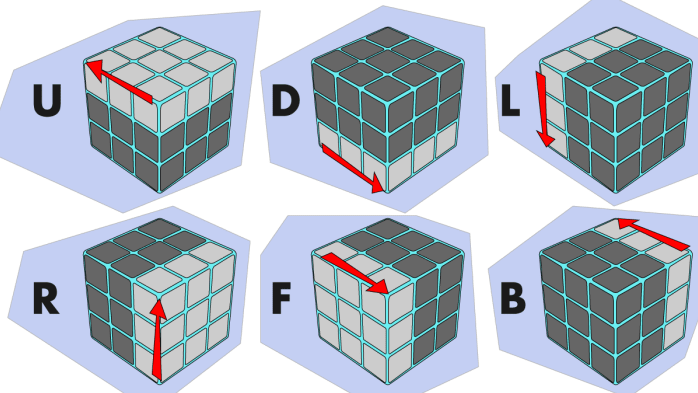
\includegraphics[scale=0.2]{1-0.png}
	\end{figure}
	\begin{enumerate}
		\item Getting the White Cross\par
		F'UL'U'
		\begin{figure}[!ht]
			\centering
			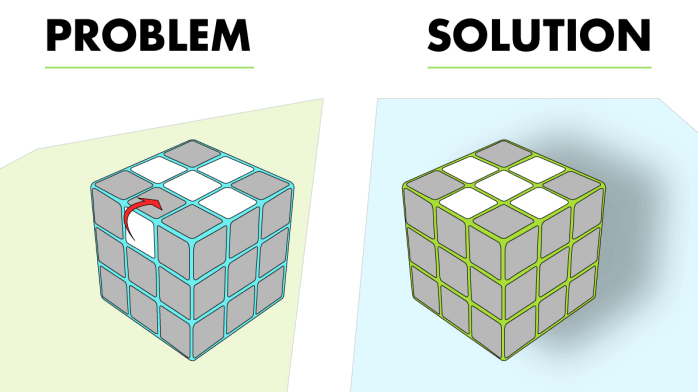
\includegraphics[scale=0.2]{1-1.png}
		\end{figure}
		\item First Layer: Left and Right Corners
		\begin{enumerate}
			\item Left corner: DLD'L'
			\item Right corner: D'R'DR
		\end{enumerate}
		\begin{figure}[!ht]
			\centering
			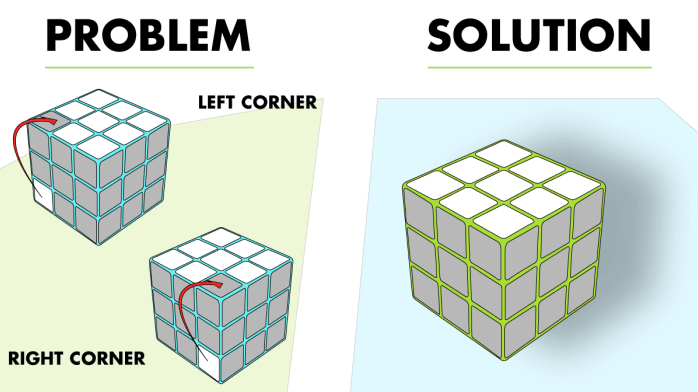
\includegraphics[scale=0.2]{1-2.png}
		\end{figure}
		\item Solving Edge-Piece Placement
		\begin{enumerate}
			\item Right edge-piece placement: URU'R'U'F'UF
			\item Left edge-piece placement: U'L'ULUFU'F'
		\end{enumerate}
		\begin{figure}[!ht]
			\centering
			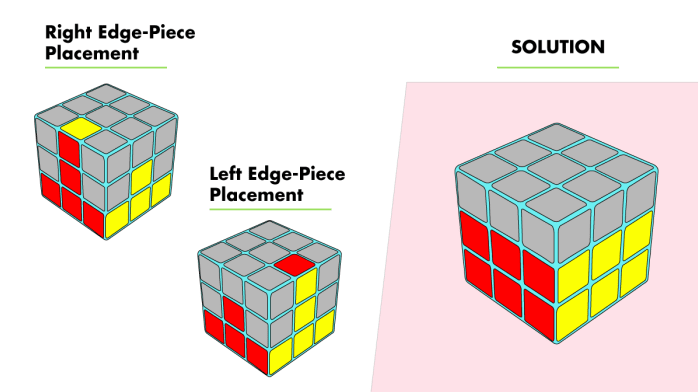
\includegraphics[scale=0.2]{1-3.png}
		\end{figure}
		\newpage
		\item Getting the White Cross Without Disrupting the Rest of the Cube\par
		FRUR'U'F'
		\begin{figure}[!ht]
			\centering
			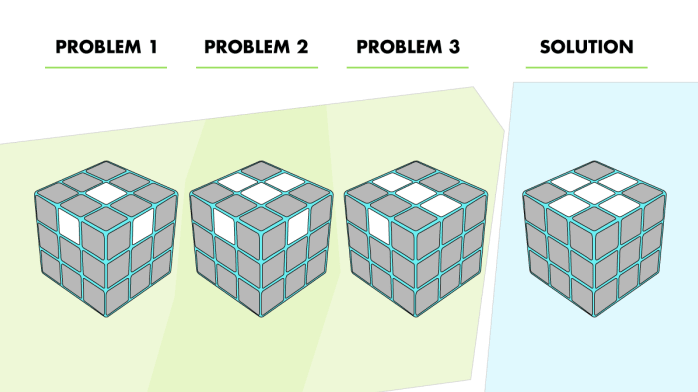
\includegraphics[scale=0.2]{1-4.png}
		\end{figure}
		\item Solving Third Layer Edge Pieces\par
		RUR'URUUR'
		\begin{figure}[!ht]
			\centering
			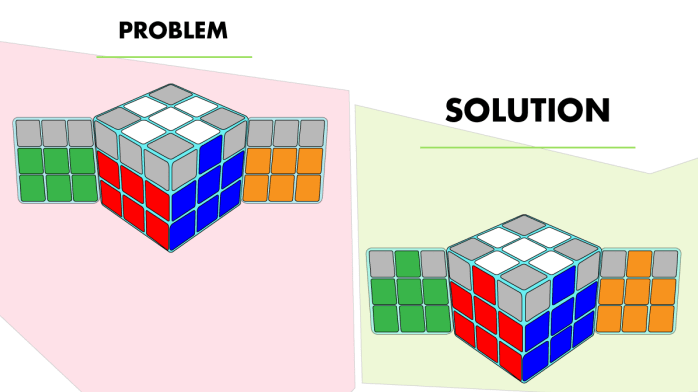
\includegraphics[scale=0.2]{1-5.png}
		\end{figure}
		\item Aligning the Third Layer Corner Pieces\par
		URU'L'UR'U'L
		\begin{figure}[!ht]
			\centering
			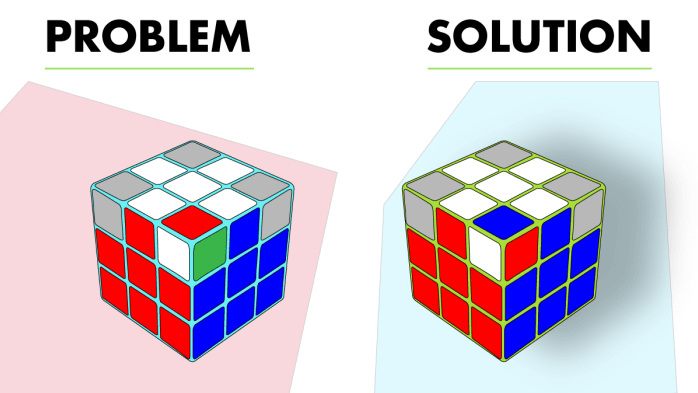
\includegraphics[scale=0.2]{1-6.png}
		\end{figure}
		\item Aligning the Corners and Finishing the Cube\par
		R'D'RD
		\begin{figure}[!ht]
			\centering
			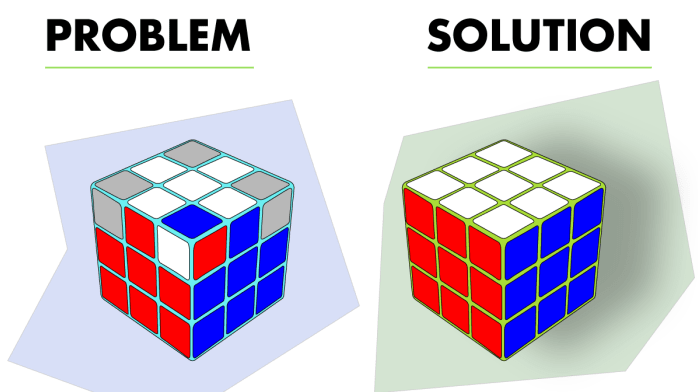
\includegraphics[scale=0.2]{1-7.png}
		\end{figure}
	\end{enumerate}
	\newpage
	\item {\bf Algorithm 2\cite{ref2}}\par
	Fridrich (CFOP) method.
	\begin{figure}[!ht]
		\centering
		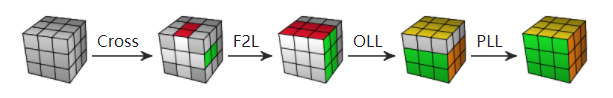
\includegraphics[scale=0.5]{2.png}
	\end{figure}
	\begin{enumerate}
		\item Cross
		\item First two layers (F2L)
		\item Orienting the last layer (OLL)
		\item Permutate the last layer (PLL)
	\end{enumerate}
\end{itemize}

\section*{Ex.4 The $\mathcal{NP}$ classes}
\begin{enumerate}
	\item We could simply use DFS to check if a given graph has a simple path, the complexity of which is $\mathcal{O}(|V|+|E|)$. Hence it is in $\mathcal{NP}$.
	\item The complexity of the simplest way that we just check from 1 to the given integer $n$ is $\mathcal{O}(n)$. Hence it is in $\mathcal{NP}$.
	\item Let us consider the reduction of vertex cover problem to {\it clique} problem\footnote{Clique of $G(V,E)$ is a subset of $V$, where each couple of vertexs is connected by one of the edges in $E$.}, which is $\mathcal{NP}$-complete, a give graph $G$ has a clique of size $k$ if and only if the complement of $G$, $\bar{G}=(V,\bar{E})$ has a vertex cover of size $|V|-k$.\par
	Assume that $G$ has a clique $V'\subseteq V$, and $|V'|=k$. Let $(u,v)$ be an arbitrary edge in $\bar{E}$, then $(u,v)\notin E$. So that at least one of $u$ and $v$ does not belong to $V'$. Equivalently, at least one of $u$ and $v$ belongs to $V\backslash V'$, i.e., $(u,v)$ is covered by $V\backslash V'$. Hence, $V\backslash V'$ size of $|V|-k$ is a vertex cover of $\bar{G}$. Vice versa.
\end{enumerate}

\section*{Ex.5 PRIMES is in $\mathcal{P}$}
The time complexity of division process\cite{ref3} is $\mathcal{O}(\log{n})$, when $n$ is sufficiently large.
\begin{lstlisting}[language=C]
int Pos_Div(int x, int y)
{
	int ans = 0;
	for (int i = log(x)/log(2); i >= 0; i--)
	{
		if ((x >> i) >= y)
		{
			ans += (1 << i);
			x -= (y << i);
		}
	}
	return ans;
}
\end{lstlisting}
According to Prime Number Theorem, the number of primes less than integer $n$ is
$$\pi(n) \sim \frac{n}{\ln{n} + B},$$
which is the times of division process. Hence the time complexity of trial division is
$$\mathcal{O}\left(\frac{\log{n}}{\ln{n}}n\right)=\mathcal{O}(\log{e}\cdot n) = \mathcal{O}(n)$$
Hence it is in $\mathcal{P}$.
\begin{thebibliography}{99}
\bibitem{ref1}https://hobbylark.com/puzzles/Rubik-Cube-Algorithms
\bibitem{ref2}https://ruwix.com/the-rubiks-cube/advanced-cfop-fridrich/
\bibitem{ref3}https://www.zhihu.com/question/47423427
\end{thebibliography}
\end{document}
